% A content fragment, meant to be \input{} or \include{}d from a master
% document that supplies \documentclass, packages (graphicx, amsmath,
% unicode-math + fontspec — compile the master with xelatex or lualatex),
% \begin{document}/\end{document}, and its own bibliography.

\section{Case Study}

The model was applied to a single adult male subject, aged 35 years, with a height h of 170 cm, observed over 130 consecutive days from 29 June to 5 November 2026. At baseline his body mass m was 94.0 kg, a body mass index of 32.5 kg/m², which falls in the World Health Organization's class I obesity range \cite{ref_who1995}; his healthy body mass m\_des was set to 70 kg, a BMI\_des of 24.2 kg/m². Over the study he weighed in daily and logged every food eaten by weight, with its macronutrients, every activity with its duration and metabolic equivalent, and his bed and wake times, so that each input of the forward model in Fig.~\ref{fig_systemdiagram} was measured rather than assumed. The daily targets were proposed by the inverse model of Fig.~\ref{fig_inversediagram} on the Mifflin-St Jeor basal metabolic rate, the Boer lean body mass, a weekly loss Δm\% of 1\% of m̄, and an 8-hour desire sleep s\_des. By the end of the study his body mass was 76.2 kg (7-day average m̄ of 76.7 kg, a BMI of 26.5 kg/m²), a loss of 17.8 kg, or 0.96 kg per week, with a U.S. Navy body-fat estimate of 22.2\% and a lean body mass of 57.4 kg. Fig.~\ref{fig_casebodymass} to Fig.~\ref{fig_casesleep} show the logged data and the model's outputs over the whole study.

\begin{figure}[htbp]
\centering
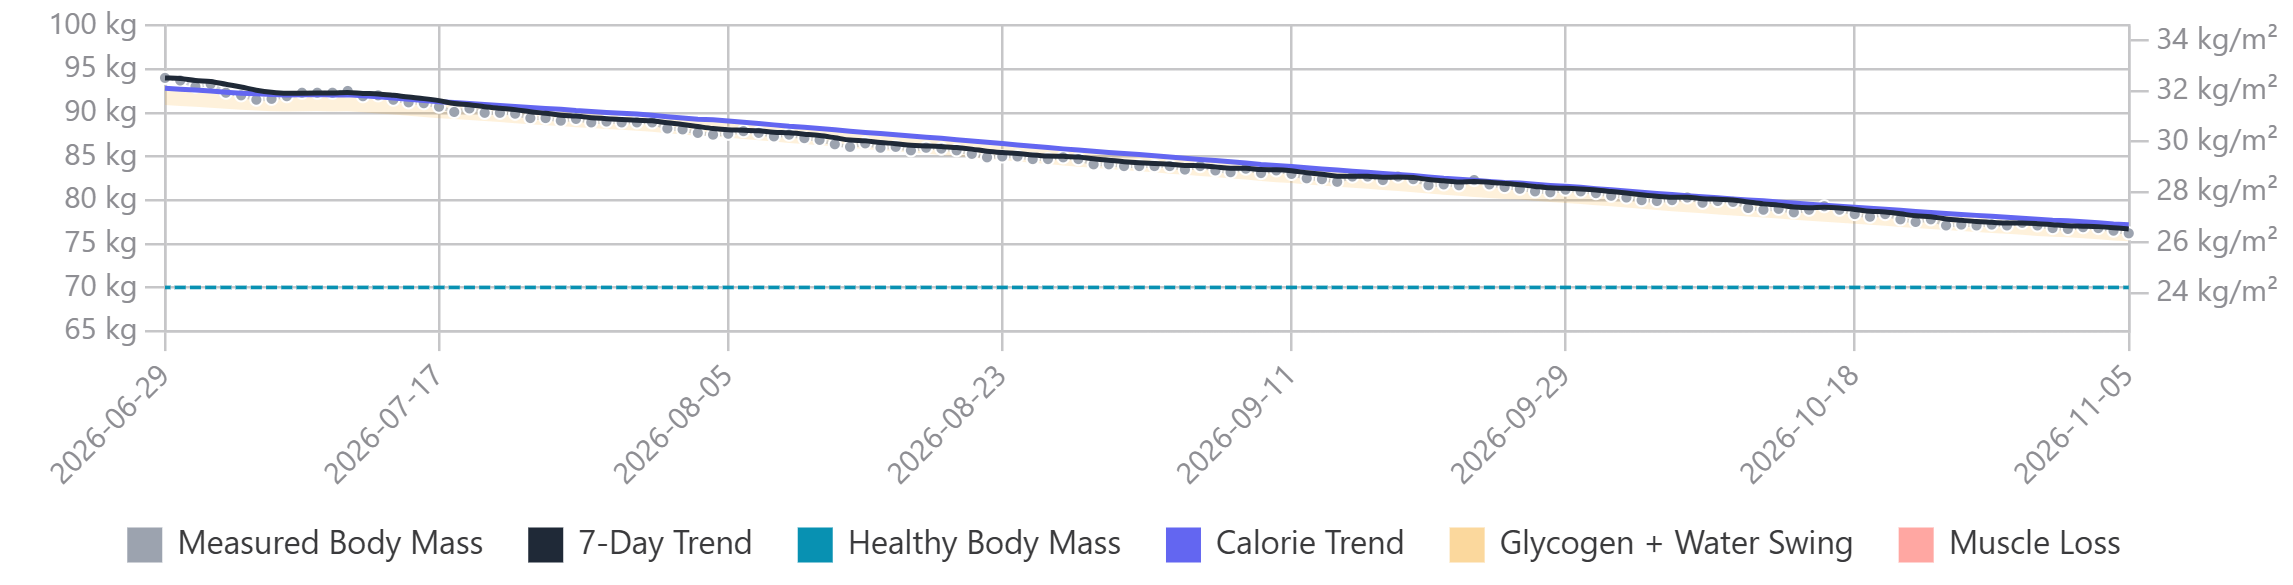
\includegraphics[width=\linewidth]{assets/figures/case-study-body-mass.png}
\caption[Body mass over the case study.]{Body mass over the 130-day case study: the measured daily body mass m (gray dots), its 7-day rolling average m̄ of eqn.~\eqref{eqn_msmo} (black), the healthy body mass m\_des of 70 kg (dashed teal), the glycogen and water swing ΔM\_gly of eqn.~\eqref{eqn_dmgl} as a band below m̄ (amber), and the calorie-implied trajectory (indigo), the body mass the logged daily energy balance alone predicts from the first day. The right axis gives the matching BMI. The calorie-implied trajectory ends at 77.2 kg against a measured m̄ of 76.7 kg, a gap of 0.5 kg after a 17.3 kg fall in m̄.}
\label{fig_casebodymass}
\end{figure}

\begin{figure}[htbp]
\centering
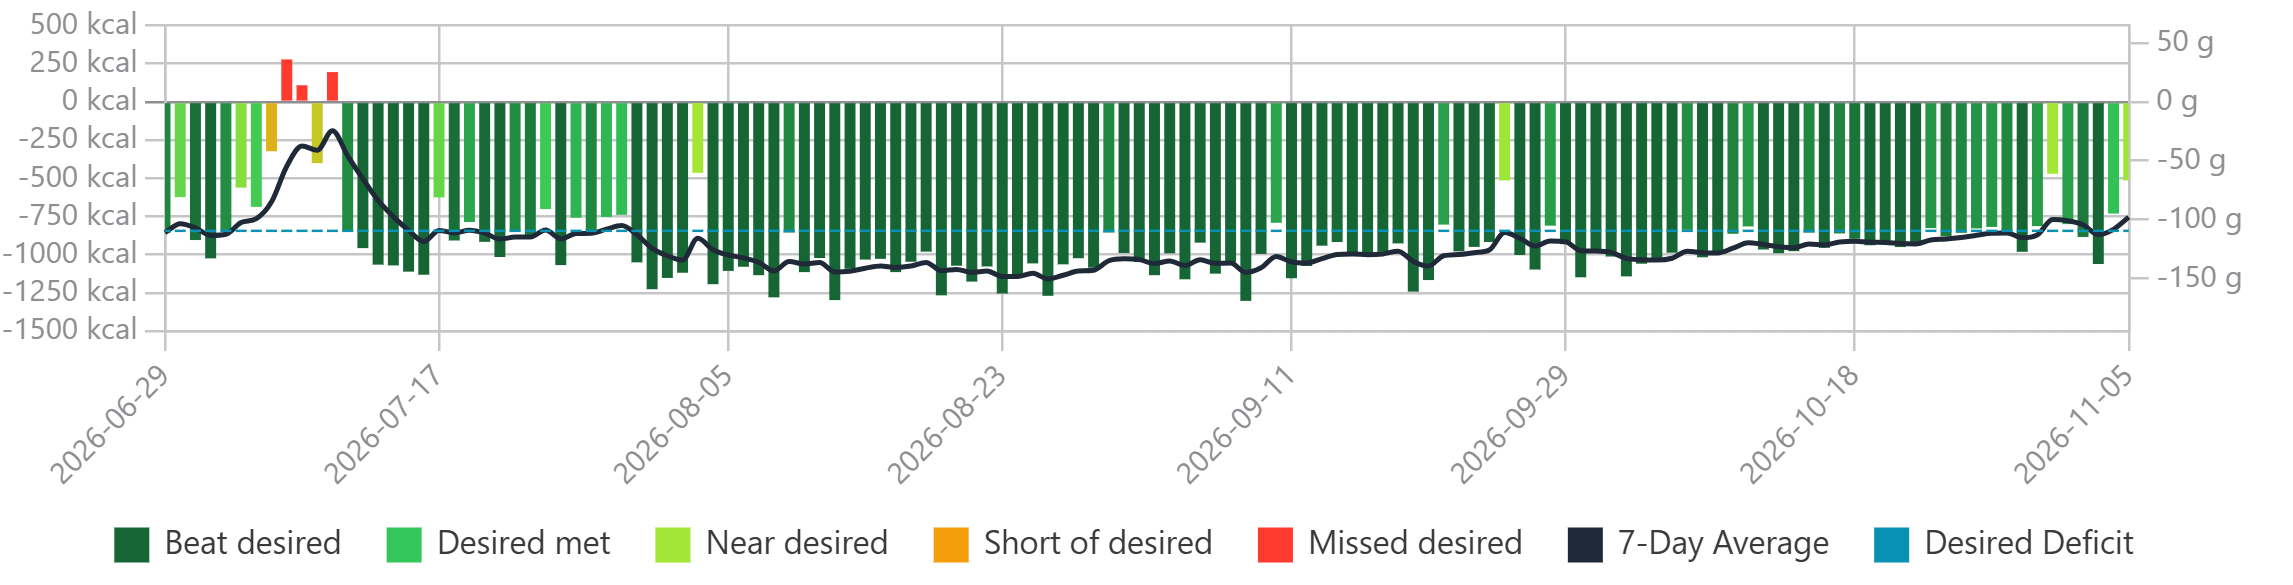
\includegraphics[width=\linewidth]{assets/figures/case-study-calorie-balance.png}
\caption[Daily calorie balance over the case study.]{Daily calorie balance TEI − BMR − AEE − TEF + SD of eqn.~\eqref{eqn_bcdi} (bars, negative for a deficit), coloured by how it compares with the desired deficit D of eqn.~\eqref{eqn_defc} (dashed teal): beat, met, near, short of or missed; its 7-day average (black); and, on the right axis, the fat-mass change in grams that balance implies at the fat energy density ρ. The balance averaged −929 kcal per day over the study.}
\label{fig_casecaloriebalance}
\end{figure}

\begin{figure}[htbp]
\centering
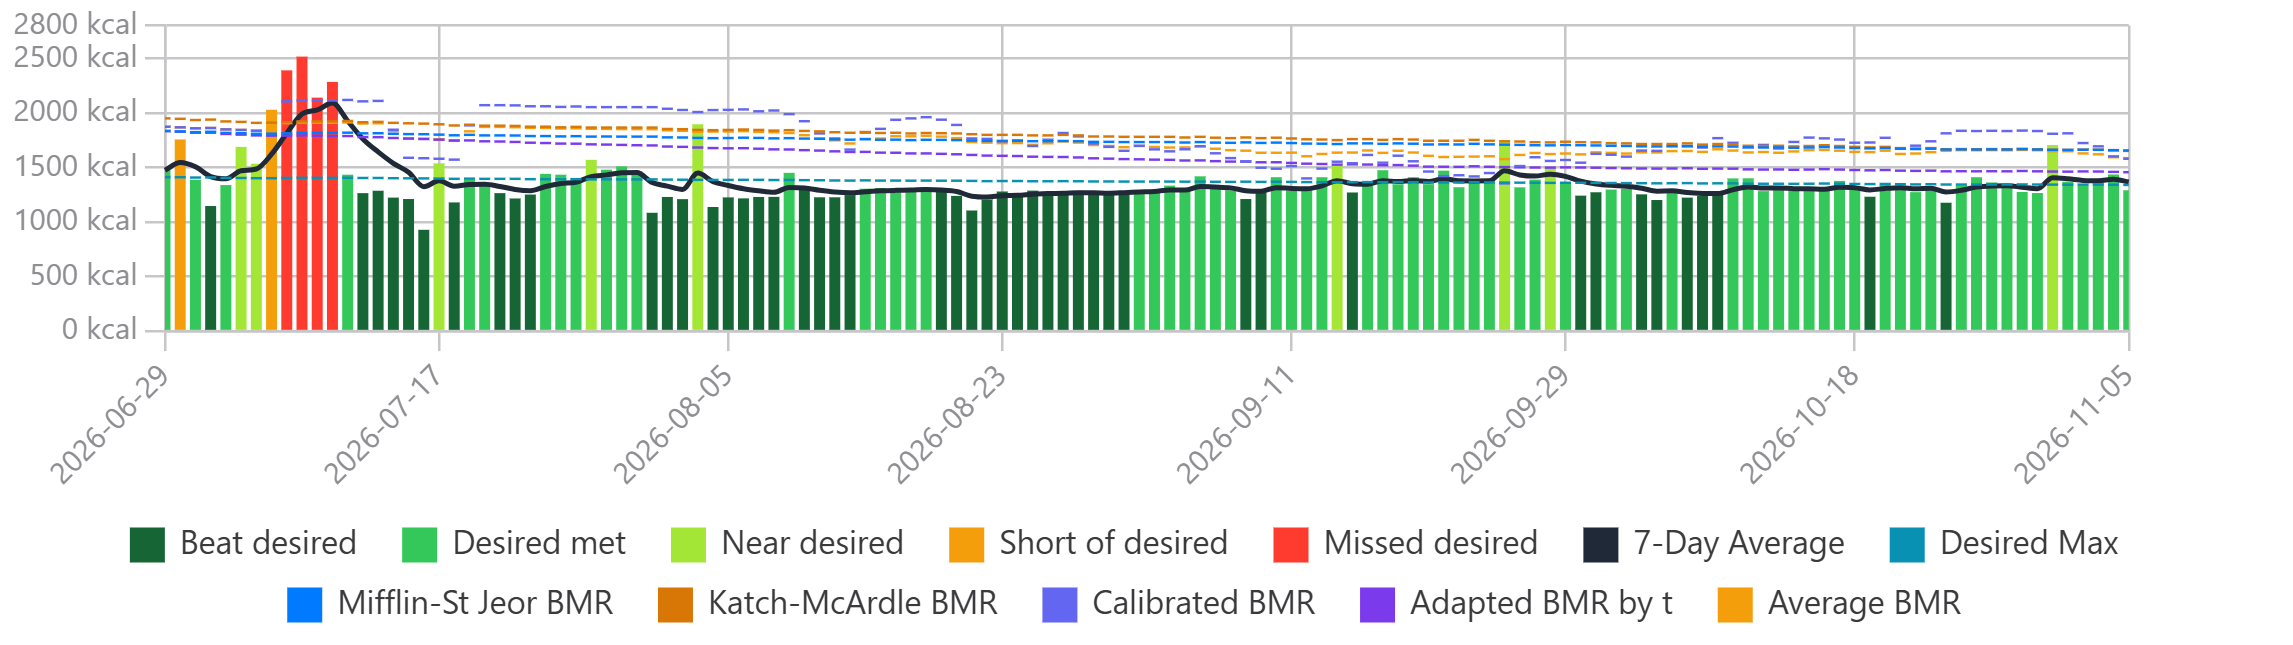
\includegraphics[width=\linewidth]{assets/figures/case-study-caloric-intake.png}
\caption[Daily energy intake against the four basal metabolic rates.]{Daily total energy intake TEI (bars), coloured by how it compares with the desired intake of eqn.~\eqref{eqn_eink}, and its 7-day average (black), set against the four basal metabolic rates of Section 4.2 as they evolved with m̄ (dashed): Mifflin-St Jeor BMR\_mif, Katch-McArdle BMR\_kat, calibrated BMR\_cal, adapted BMR\_adp, and their average BMR\_avg. Intake averaged 1,366 kcal per day, below every estimate of BMR; the gap is D\_bmr\% of eqn.~\eqref{eqn_dbmr}.}
\label{fig_casecaloricintake}
\end{figure}

\begin{figure}[htbp]
\centering
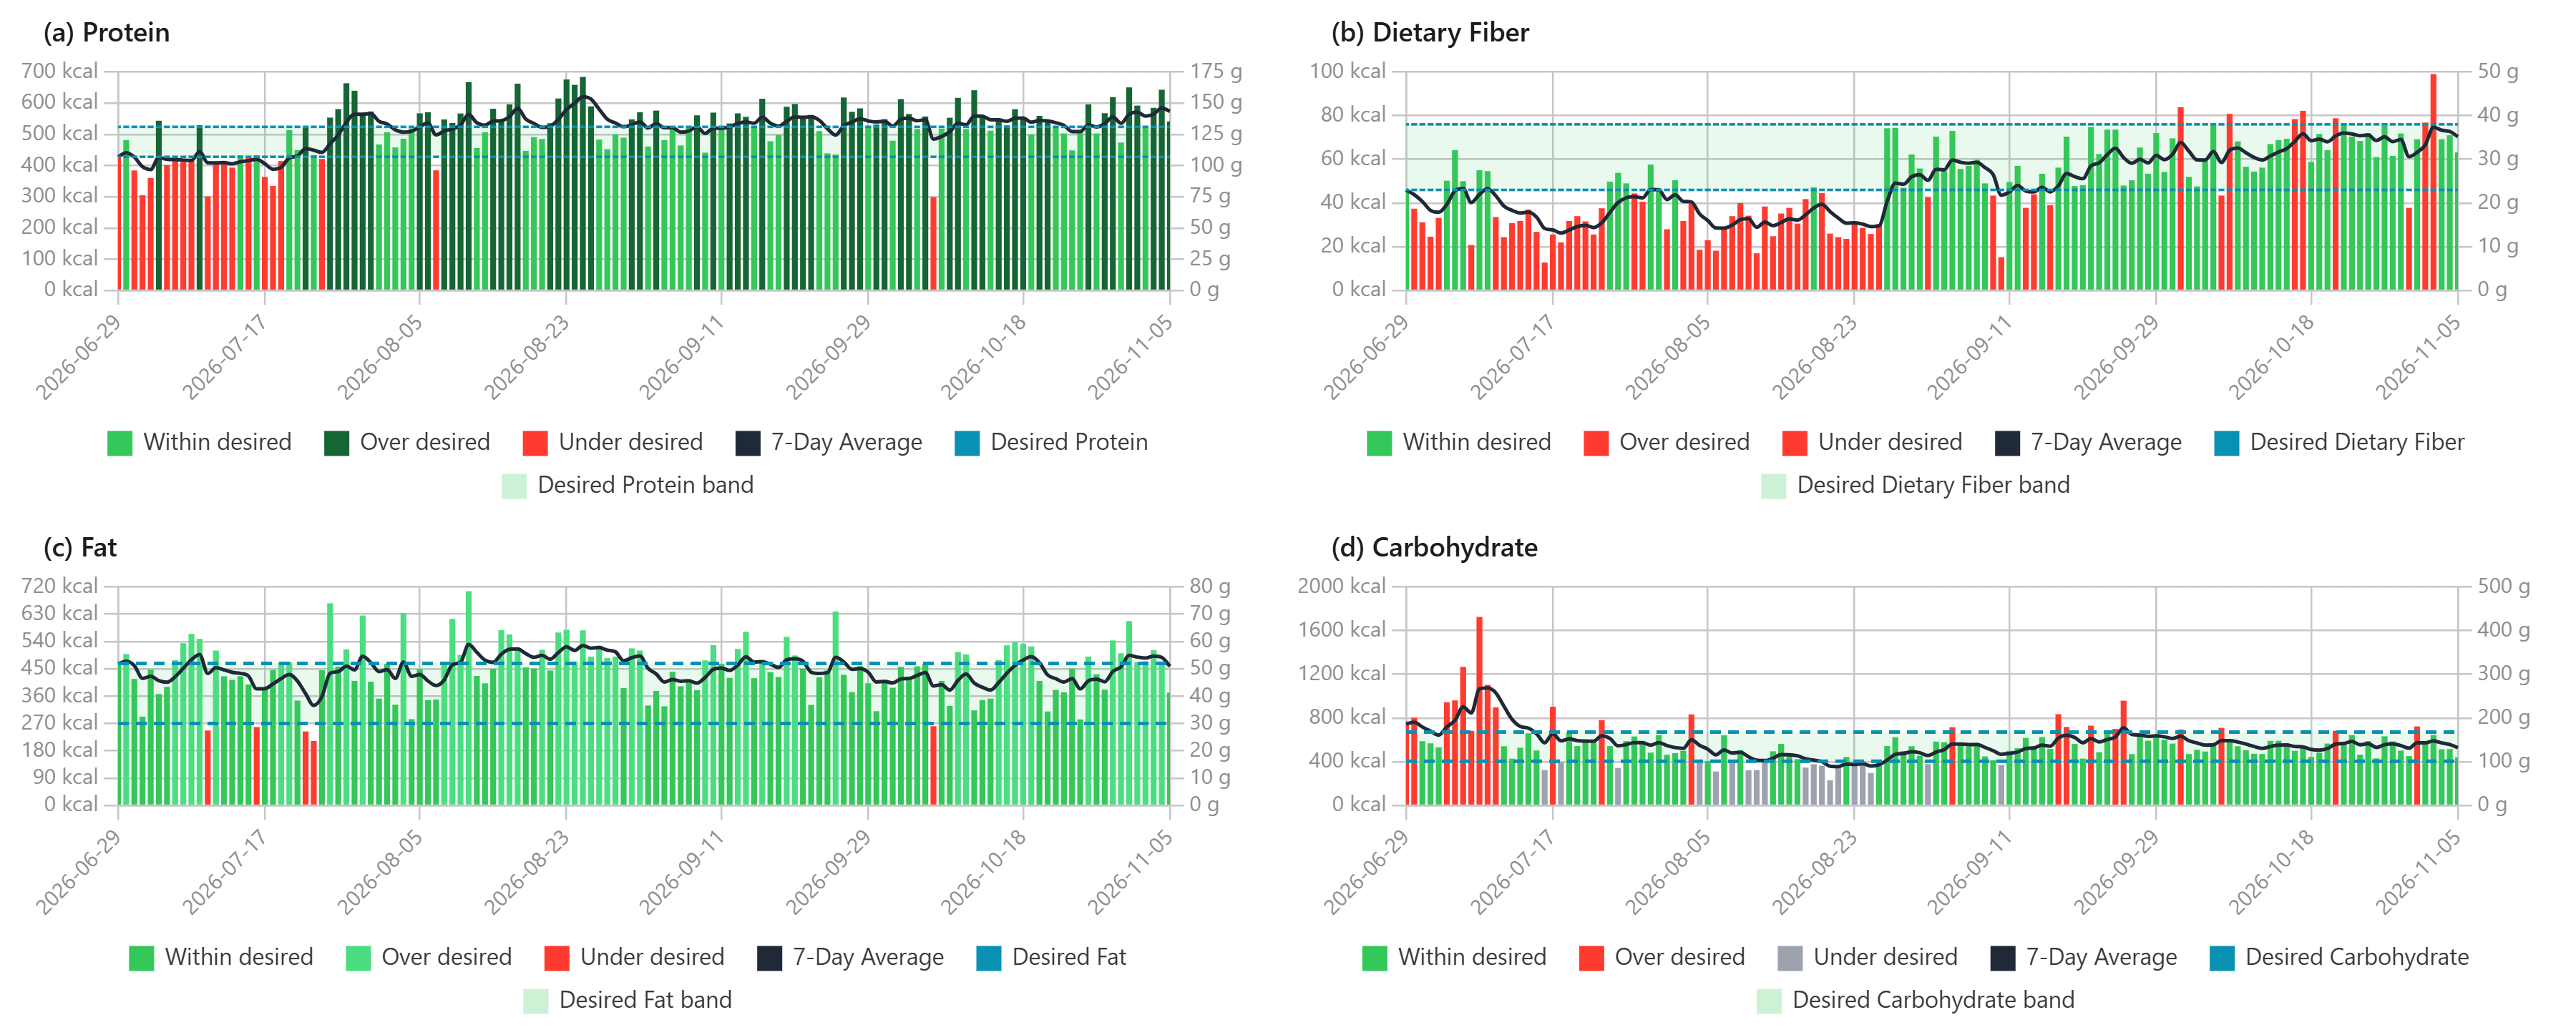
\includegraphics[width=\linewidth]{assets/figures/case-study-macronutrients.png}
\caption[Daily macronutrient intake against the dietary requirement bands.]{Daily intake of (a) protein, (b) dietary fiber, (c) fat and (d) carbohydrate, in grams on the right axis and in kcal on the left, each against its healthy band from Section 5 (shaded, between the dashed lines): P\_min to P\_max of eqns.~\eqref{eqn_pmin}–\eqref{eqn_pmax}, F\_min to F\_max of eqns.~\eqref{eqn_fmin}–\eqref{eqn_fmax}, G\_min to G\_max of eqns.~\eqref{eqn_gmin}–\eqref{eqn_gmax}, and C\_min to C\_max of eqns.~\eqref{eqn_cmin}–\eqref{eqn_cmax}. Bars are coloured within, over or under the band, with each 7-day average in black.}
\label{fig_casemacronutrients}
\end{figure}

\begin{figure}[htbp]
\centering
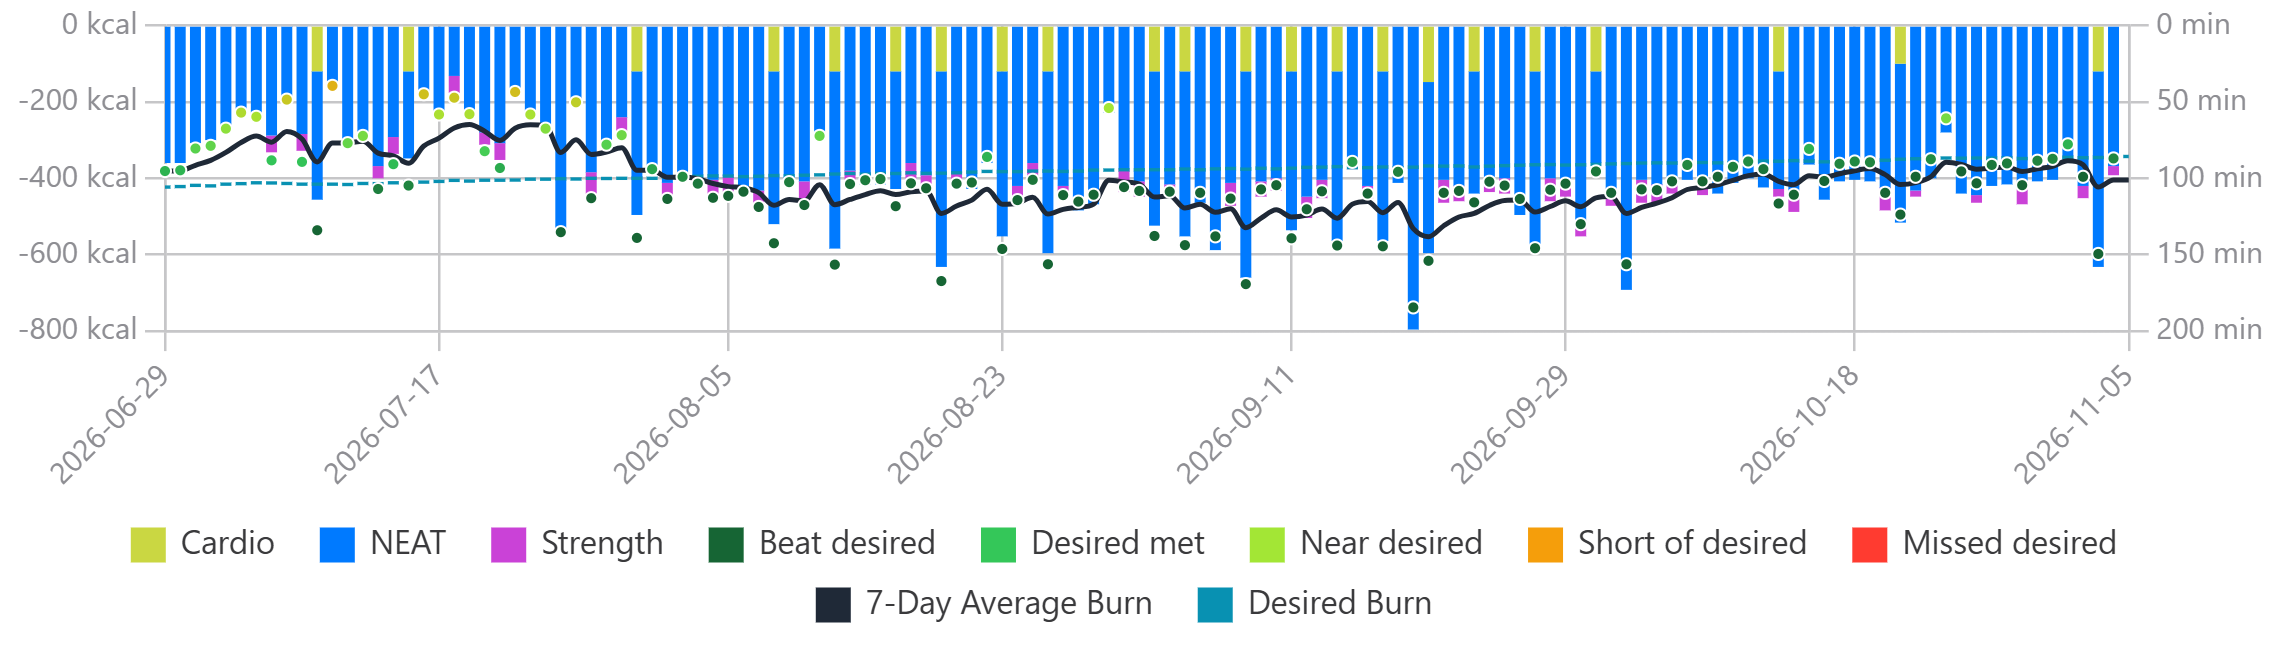
\includegraphics[width=\linewidth]{assets/figures/case-study-physical-activity.png}
\caption[Daily activity energy expenditure over the case study.]{Daily activity energy expenditure AEE of eqn.~\eqref{eqn_eact}, split into cardio, non-exercise activity thermogenesis (NEAT) and strength (stacked bars, drawn downward as energy out), with the day's total coloured by how it compares with the desired burn (dots), its 7-day average (black) and the desired burn itself (dashed teal); the right axis gives the active duration τ.}
\label{fig_casephysicalactivity}
\end{figure}

\begin{figure}[htbp]
\centering
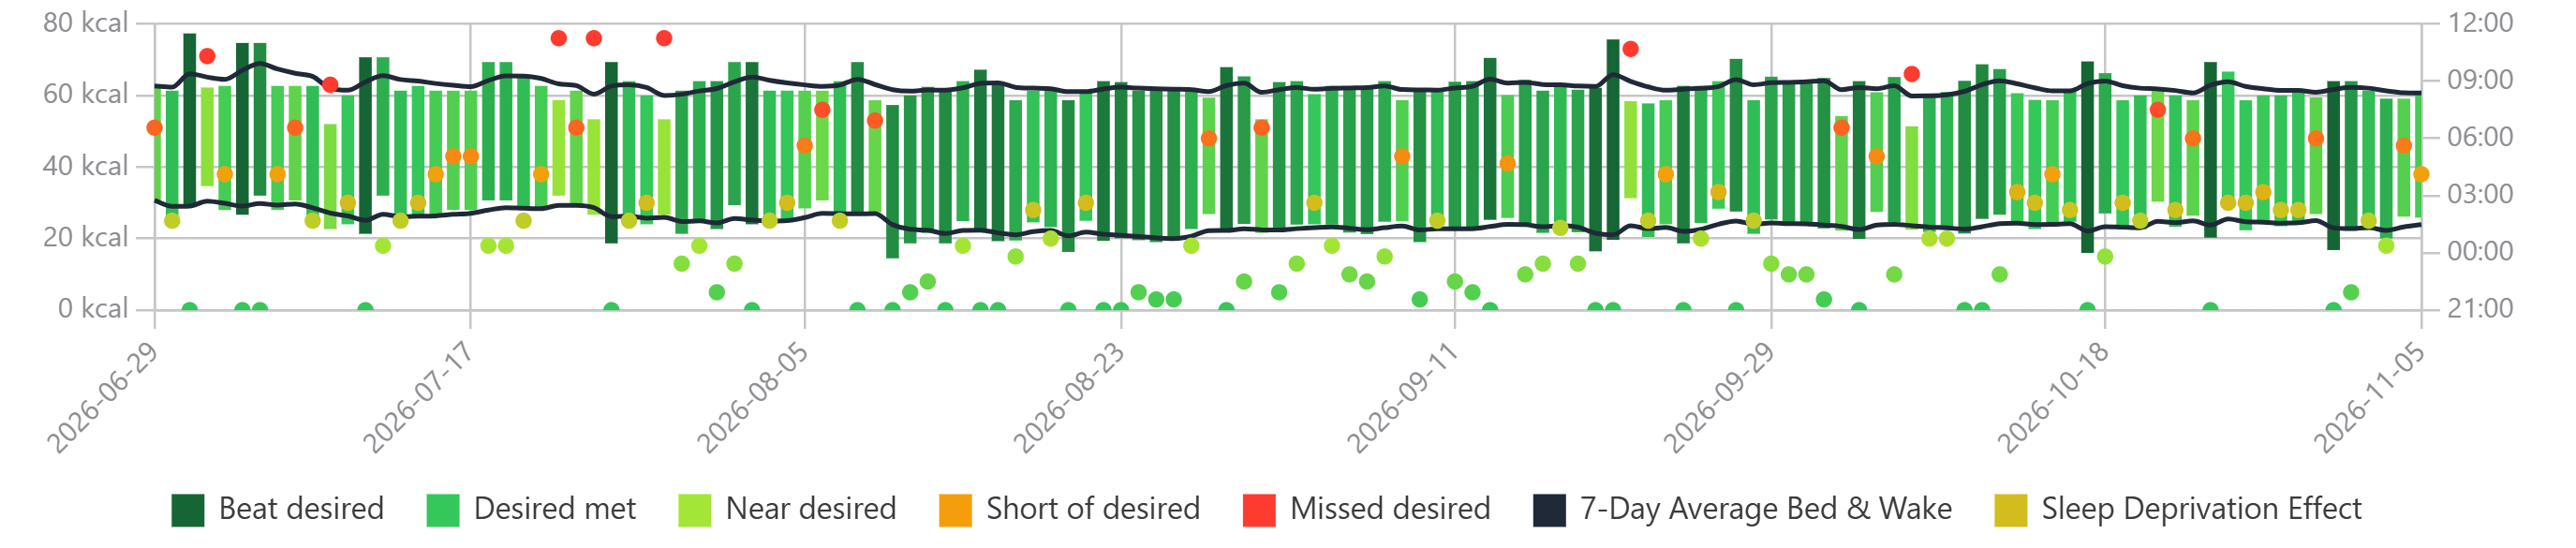
\includegraphics[width=\linewidth]{assets/figures/case-study-sleep.png}
\caption[Sleep over the case study.]{Nightly sleep, each bar spanning bed to wake time on the right axis and coloured by its length s against the 8-hour desire sleep s\_des; the 7-day average bed and wake times (black); and, on the left axis, the sleep deprivation effect (dots), the energy a short night costs the day's deficit through the sleep efficiency factor η of eqn.~\eqref{eqn_slef}.}
\label{fig_casesleep}
\end{figure}
